\section{国内外研究现状}
\subsection{仿生机器鼠研究现状}
生物鼠形体轻巧,行动灵活,表现出优秀的地形适应能力,激发了研究者开发仿生多足移动机器人的灵感。但由于早期研究者设计四足仿生机器鼠时面临着驱动器和控制器集成、小型机器人四足步态规划等难题,较早成熟的仿生机器鼠大多为轮式结构。其中以日本早稻田大学Takanishi实验室开发的WM(Waseda Mouse)系列仿生机器鼠(图\ref{figure_wm})较为典型。
\begin{figure}[htbp]
  %\vspace{10pt} % 调整图片与上文的垂直距离
  \centering
  \subfigure[WM-2\cite{takanishiInteractionCreatureRobot1998}]{
  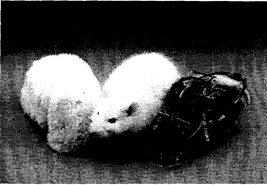
\includegraphics[height=0.18\linewidth]{images/ch01/WM2.png} \label{figure_wm2}% label 用来在文中索引
  }
  \subfigure[WM-4\cite{aokiInteractionRatRatrobots1999}]{
  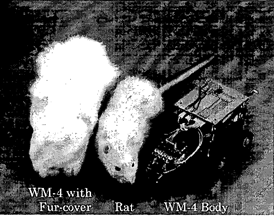
\includegraphics[height=0.18\linewidth]{images/ch01/WM4.png} \label{figure_wm4}% label 用来在文中索引
  }
  \subfigure[WM-6\cite{ishiiExperimentalStudyAutomatic2005}]{
  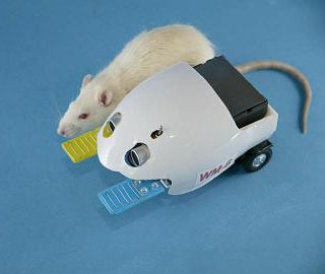
\includegraphics[height=0.18\linewidth]{images/ch01/WM6.jpg} \label{figure_wm6}% label 用来在文中索引
  }
  \subfigure[WM-8\cite{ishiiStressExposureUsing2012}]{
  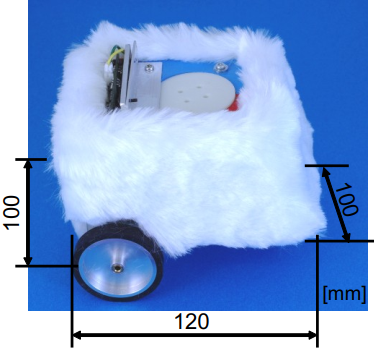
\includegraphics[height=0.18\linewidth]{images/ch01/WM8.png} \label{figure_wm8}% label 用来在文中索引
  }
  \caption{部分WM系列仿生机器鼠} \label{figure_wm}
\end{figure}
这一系列仿生机器鼠尺寸均与成年鼠相近,装备有红外传感器用于探测生物鼠和其他环境障碍,具备两个后置的驱动轮,使用者可以通过蓝牙对其运动进行控制\cite*{takanishiInteractionCreatureRobot1998, aokiInteractionRatRatrobots1999,  ishiiExperimentalStudyAutomatic2005, ishiiStressExposureUsing2012}。WM-2型仿生机器鼠由两个前置的转向轮控制方向,而随后WM-4型仿生机器鼠对两个驱动轮分别控制,使其能够进行差速运动,进而实现任意线速度和角速度的运动,这不仅提高了改型仿生机器鼠的灵活性,而且使得原本用于转向的前轮改为仅需提供支撑的万向轮,简化了仿生机器鼠的结构\cite{aokiInteractionRatRatrobots1999}。在后续的研究中,他们更新了WM-6的驱动器,并改进了外形,新的WM-8型仿生机器鼠在最大角速度上大幅超过WM-6,并且外形与生物鼠更相似\cite{ishiiStressExposureUsing2012}。

近年来,随着电机和控制器的小型化,将其集成在小型移动机器平台上成为可能。同时,人们对生物鼠的运动机理揭示逐渐深入,为仿生机器鼠的设计提供了思路。近年来,四足仿生机器鼠成为热点之一。日本和意大利的研究者们共同开发的一款仿生机器鼠全身具有12个自由度\cite{laschiDesignDevelopmentLegged2006a},能够执行前进、转向、推动杠杆和按下按钮等简单的动作,但由于其采用钢丝-滑轮驱动,运动精度较低。而日本早稻田大学自2009年开始其四足仿生机器鼠WR(Waseda Rat)系列(图\ref{figure_wr})的研究。
\begin{figure}[htbp]
  %\vspace{13pt} % 调整图片与上文的垂直距离
  \centering
  \subfigure[WR-1\cite{ishiiDevelopmentQuadrupedAnimaroid2009}]{
  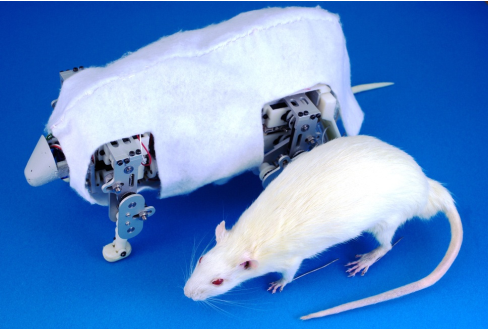
\includegraphics[height=0.2\linewidth]{images/ch01/WR1.png} \label{figure_wr1}
  }
  \subfigure[WR-2\cite{ishiiDesignDevelopmentBiomimetic2009}]{
  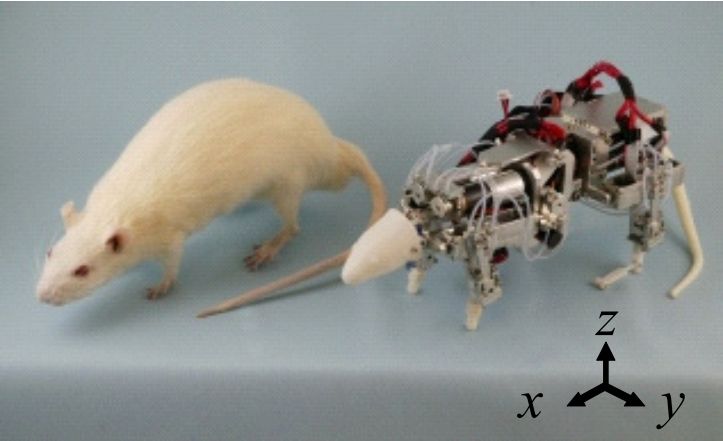
\includegraphics[height=0.2\linewidth]{images/ch01/WR2.png} \label{figure_wr2}
  }\\
  \subfigure[WR-3\cite{shiDevelopmentHybridWheellegged2010, shiDevelopmentHybridWheelLegged2011, ishiiNovelMethodDevelop2013}]{
  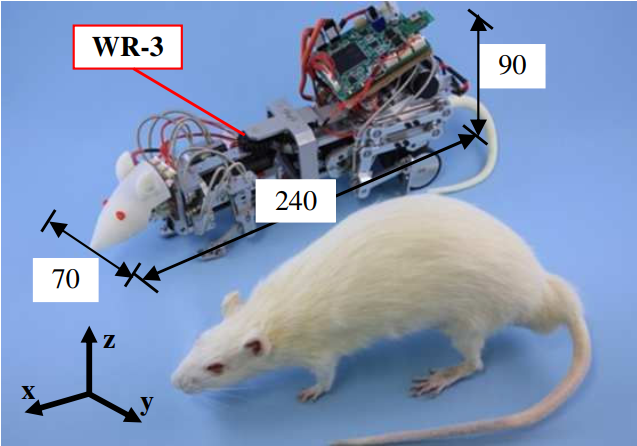
\includegraphics[height=0.2\linewidth]{images/ch01/WR3.png} \label{figure_wr3}
  }
  \subfigure[WR-4\cite{shiRobotratInteractionExperimental2011a}]{
  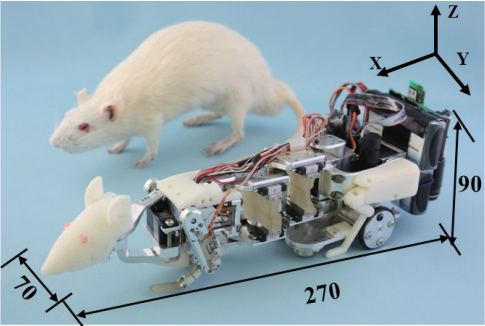
\includegraphics[height=0.2\linewidth]{images/ch01/WR4.png} \label{figure_wr4}
  }
  \subfigure[WR-5\cite{shiBehaviorModulationRats2015a}]{
  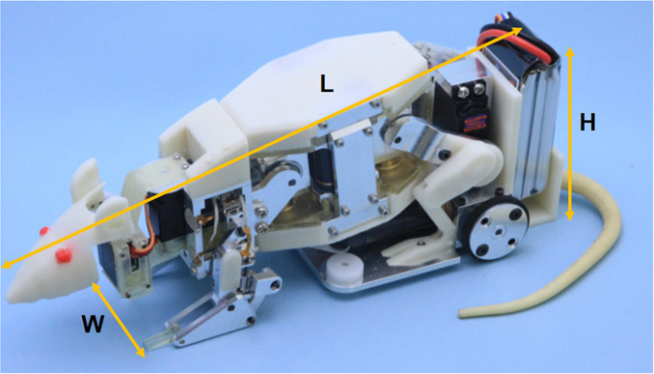
\includegraphics[height=0.2\linewidth]{images/ch01/WR5.png} \label{figure_wr5}
  }
  \caption{WR系列仿生机器鼠} \label{figure_wr}
\end{figure}
该系列仿生机器鼠每条腿均有2个主动自由度和1个被动自由度\cite*{ishiiDevelopmentQuadrupedAnimaroid2009, ishiiDesignDevelopmentBiomimetic2009, shiDevelopmentHybridWheellegged2010, shiRobotratInteractionExperimental2011a, shiDevelopmentHybridWheelLegged2011, ishiiNovelMethodDevelop2013, shiBehaviorModulationRats2015a},尽管WR-1和WR-2在产生仿鼠动作方面有不俗的表现,可以执行部分生物间交互动作,但由于其质量均远超生物鼠(约为其3倍),且运动性能不佳,最大速度仅为2-3 cm/s\cite*{ishiiDevelopmentQuadrupedAnimaroid2009, ishiiDesignDevelopmentBiomimetic2009},因此其交互性能受到局限。与前两代相比,WR-3采用轮-腿复合结构,不仅对尺寸进行了优化,还对前肢结构进行了设计,能够完成梳理等典型生物鼠动作\cite{shiDevelopmentHybridWheellegged2010},该型号仿生机器鼠在仿鼠运动方面取得了较大的发展。其后的WR-4仿生机器鼠共有12个主动自由度,运动更加灵活。在此基础上,WR-5针对仿生机器鼠的外形进行了改进,并针对腰部连接进行了模块化设计,WR-5重0.8 kg,具有13个自由度,大大提升了模仿生物鼠动作的能力\cite{shiBehaviorModulationRats2015a}。随着对生物鼠运动机理的进一步揭示,研究人员在WR-5的基础上进行了改进,根据生物鼠的运动情况设置仿生机器鼠的自由度,改进后的WR-5M在俯仰、偏向等运动模式方面均表现出与生物鼠相近的性质\cite{shiModifiedRoboticRat2018}。

除WR系列仿生机器鼠外,德国慕尼黑工业大学也对仿生机器鼠进行了研究。其开发的NRP系列仿生机器鼠(图\ref{figure_tum})利用弹簧机构模拟生物鼠腿部肌腱,实现仿鼠行走运动\cite{lucasDesignBiomimeticRodent2018}。
\begin{figure}[htbp]
  %\vspace{0pt} % 调整图片与上文的垂直距离
  \centering
  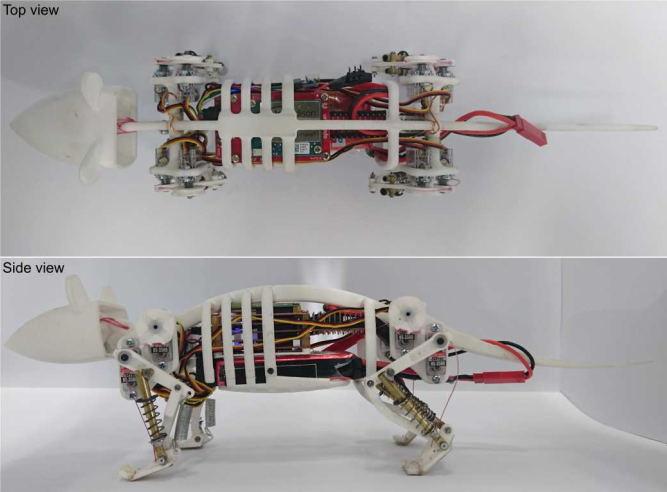
\includegraphics[width=0.5\linewidth]{images/ch01/tum.png}
  \caption{慕尼黑工业大学仿生机器鼠}\label{figure_tum} % label 用来在文中索引
\end{figure}

对仿生机器鼠腰部结构的设计是另一难点。一般认为,生物鼠腰部对其实现前身俯仰和偏航运动具有重要作用,因此必须具备至少2个自由度\cite{shiDevelopmentHybridWheellegged2010},早期的仿生机器鼠均不具备腰部运动的能力\cite{ishiiStressExposureUsing2012, ishiiDesignDevelopmentBiomimetic2009, ishiiDevelopmentQuadrupedAnimaroid2009, shiModulationRatBehaviour2013},限制着仿生机器鼠产生仿鼠运动,这一情况到2009年得以改善,早稻田大学的研究人员设计的WR-3仿生机器鼠具备2个腰部自由度,但这一设计为其腿部运动的稳定性,尤其是产生直立动作时带来了挑战,为克服这一困难,他们采取了轮-腿复合结构,并在WR-4中沿用这一设计\cite{shiDevelopmentHybridWheellegged2010, shiRobotratInteractionExperimental2011a, shiDevelopmentHybridWheelLegged2011}。而NRP系列仿生机器鼠采用弹簧四肢结构和鼠尾辅助支撑实现直立动作,因此未设置腰部自由度,这也使得其转弯半径高达30-40 cm,灵活度较差\cite{lucasDesignBiomimeticRodent2018}。

国内仿生机器鼠设计也有一定成果。东北大学设计的四轮仿生机器鼠(图\ref{figure_cn}\subref{figure_nerat})具有一定的在筛网状地面行走和进入小洞的能力,但并不具备任何生物鼠特有的动作特性\cite{guoFangShengShuJiJieXiTongSheJiYuYunDongTeXingYanJiu2010}。徐若愚等设计的机械小鼠(图\ref{figure_cn}\subref{figure_xurat})通过添加一系列感应装置实现仿鼠行为,包括觅食、逃避和自我保护等\cite{xuFangShengJiJieXiaoShuDeYanJiuJiSheJi2016}。我们对日本早稻田大学的WR-5仿生机器鼠进行了改进得到WR-5M(图\ref{figure_cn}\subref{figure_lirat}),优化设计了前肢机构及控制电路板,使得该仿生机器鼠在外形上更接近生物鼠,同时能够更好地模仿生物鼠的前肢运动,在最大俯仰角(MPA)和最大到达高度(MRH)、最大弯曲角(MBA)和最小弯曲距离(MBD)4个参数的评估中均有较大改善\cite{liJiQiShuDeFangShuYunDongChengDuPingGu2017a}。
\begin{figure}[htbp]
  %\vspace{13pt} % 调整图片与上文的垂直距离
  \centering
  \subfigure[东北大学四轮仿生机器鼠\cite{guoFangShengShuJiJieXiTongSheJiYuYunDongTeXingYanJiu2010}]{
  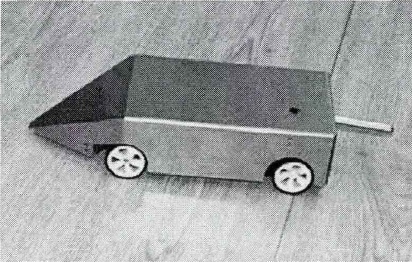
\includegraphics[height=0.18\linewidth]{images/ch01/nerat.png} \label{figure_nerat}
  }
  \subfigure[徐若愚机械小鼠\cite{xuFangShengJiJieXiaoShuDeYanJiuJiSheJi2016}]{
  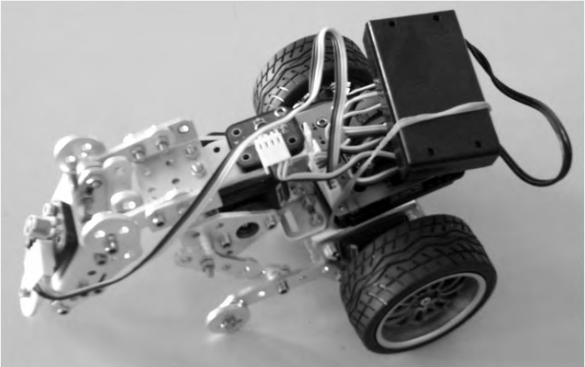
\includegraphics[height=0.18\linewidth]{images/ch01/xurat.png} \label{figure_xurat}
  }
  \subfigure[WR-5M仿生机器鼠\cite{liJiQiShuDeFangShuYunDongChengDuPingGu2017a}]{
  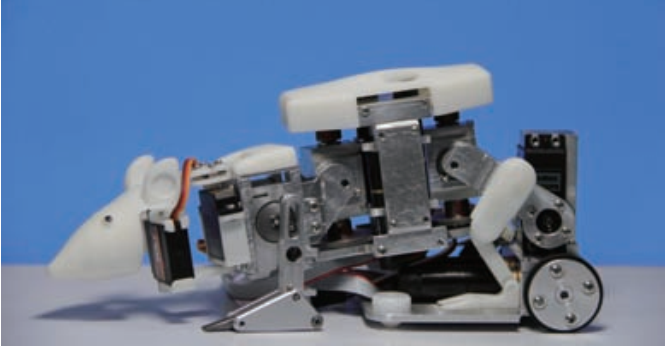
\includegraphics[height=0.18\linewidth]{images/ch01/lirat.png} \label{figure_lirat}
  }
  \caption{国内仿生机器鼠研究} \label{figure_cn}
\end{figure}

综合以上研究,目前仿生机器鼠经历了从轮式到足式,从腰部固连到设置多个腰部自由度的过程,其发展具有明显的小型化和智能化的趋势,与生物鼠的外形差距在不断减小。随着对生物鼠机理的进一步揭示,仿生机器鼠结构和运动将得到不断优化,其行为产生、智能控制和决策领域将受到研究者进一步重视,而仿生机器鼠与生物鼠的行为交互即是这一领域的重要研究方向。

\subsection{仿生机器鼠交互研究}
作为一种典型的模式动物,生物鼠的行为表现与其内部情绪变化、个体生理属性即外部环境状态有着密切联系。揭示生物鼠行为变化,尤其是多只生物鼠交互时的变化规律,对揭示其上述生物特性有着重要意义,因而受到研究者的广泛关注。但由于生物的不可控性,在研究过程中,科学家一直试图寻找一种便于操控的仪器作为生物鼠的交互对象。仿生机器鼠的出现为此提供了一种选择,设计精巧的仿生机器鼠皆能够产生与生物鼠相似的动作和行为,进而诱发生物鼠的交互反应,又能够被科学家精确控制。在研究仿生机器鼠结构和控制方式的过程中,研究者们也一直在关注其在动物交互实验过程中的作用。

WM系列仿生机器鼠的研究团队利用其成果进行了部分社交试验。他们利用WM-2研究仿生机器鼠对生物鼠行为的影响,在实验的前半部分,生物鼠对仿生机器鼠表现出经常性的嗅探和跟随行为;随着实验进行,生物鼠表现出与仿生机器鼠齐头并进的行为,这表明仿生机器鼠的部分行为能够被生物鼠认知并影响生物鼠的行为\cite{takanishiInteractionCreatureRobot1998}。但这一实验只研究了距离这一单一变量,且其焦点为生物鼠与仿生机器鼠之间的信息交流,因而对内部的生物机理揭示不足。
随后,他们利用WM-4型仿生机器鼠研究其是否能够引导生物鼠的某些行为,在实验中,WM-4与生物鼠同时寻找食物,当仿生机器鼠寻找到食物后,主动引导生物鼠前往食物位置。实验发现,当WM-4重复这一引导行为后,生物鼠受到影响,跟随WM-4并找到食物\cite{aokiInteractionRatRatrobots1999}。除此以外,\citeauthor{ishiiExperimentalStudyTask2006}提出了一种新的算法策略(图\ref{figure_wminteract}\subref{figure_wm6teach})对WM-6的接近、推杆等动作进行了训练,结果发现这一算法能够有效地对生物鼠的觅食行为进行示教\cite{ishiiExperimentalStudyTask2006}。而随后利用WM-8进行的对生物鼠的压力测试(图\ref{figure_wminteract}\subref{figure_stressEx})发现未成年生物鼠在遭受仿生机器鼠的压力时表现出比成年生物鼠更低的活力\cite{ishiiStressExposureUsing2012},这也表明仿生机器鼠可以作为研究生物鼠精神状态的良好工具。
\begin{figure}[htbp]
  %\vspace{13pt} % 调整图片与上文的垂直距离
  \centering
  \subfigure[WM-6仿生机器鼠行为生成算法\cite{ishiiExperimentalStudyTask2006}]{
  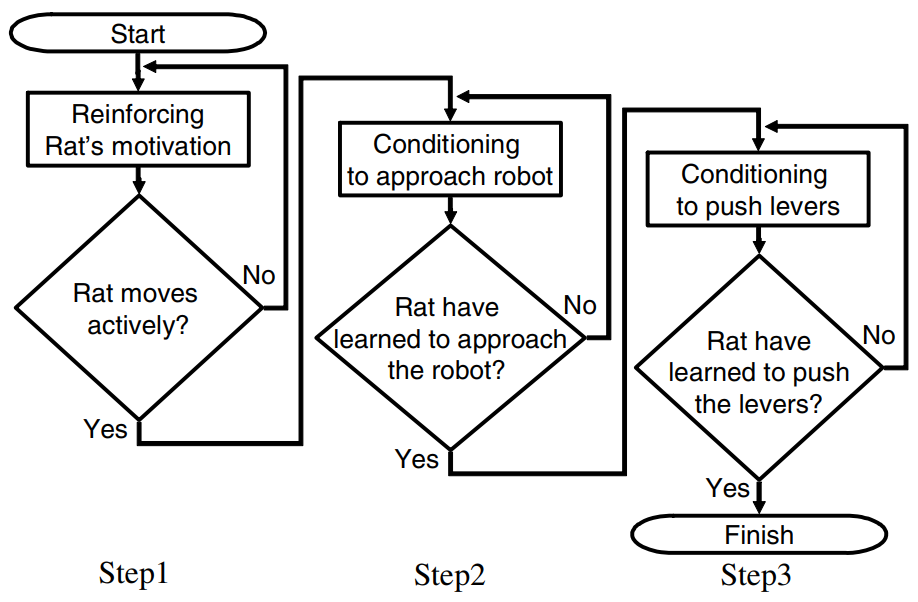
\includegraphics[height=0.3\linewidth]{images/ch01/WM6teach.png} \label{figure_wm6teach}
  }
  \subfigure[WM-8对生物鼠进行压力测试的实验装置\cite{ishiiStressExposureUsing2012}]{
  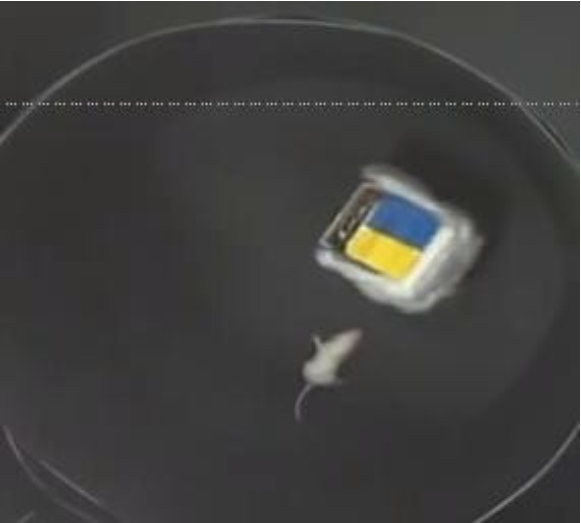
\includegraphics[height=0.3\linewidth]{images/ch01/StressEx.png} \label{figure_stressEx}
  }
  \caption{部分WM系列仿生机器鼠行为交互实验} \label{figure_wminteract}
\end{figure}

研究人员同样利用WR仿生机器鼠开展了一系列交互实验,\citeyear{laschiDesignDevelopmentLegged2006a}年,
开发团队尝试利用四足仿生机器鼠示教生物鼠执行特定的动作后获取食物\cite{laschiDesignDevelopmentLegged2006a}。WR-3具有优秀的产生仿鼠运动的能力,他们将生物鼠的运动阶段分为移动和交互两个过程,控制仿生机器鼠产生直立、转身、梳理和爬上等行为,在交互实验中生物鼠对仿生机器鼠由戒备逐渐变为友好,这表明仿生机器鼠的特定社交行为能够诱使生物鼠模仿其行为。\cite{shiDevelopmentHybridWheellegged2010}。

随后,他们利用WR-4与生物鼠进行了社交反应测试,在实验中,WR-4在第一阶段表现跟随行为(5 $min$),之后不再运动(5 $min$),将第二阶段生物鼠表现直立行为的频率和与WR-4的距离作为观测结果,发现与WR-4交互后,生物鼠表现直立的频率明显提高,表明WR-4能够明显地影响生物鼠的行为\cite{shiRobotratInteractionExperimental2011a}。这一结论随后由WR-5M得到了证实,当WR-5M表现出与生物鼠相似的俯仰和偏向动作时,生物鼠通常随之表现出一致的动作(图\ref{figure_wr5minter}),表明机器鼠具有欺骗生物鼠并诱使其产生特定行为的能力\cite{shiModifiedRoboticRat2018}。但这些实验往往存在着持续时间短,交互模式单一等问题。
\begin{figure}[htbp]
  %\vspace{13pt} % 调整图片与上文的垂直距离
  \centering
  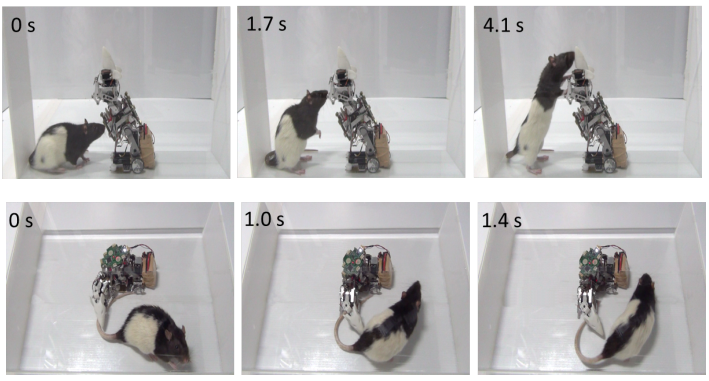
\includegraphics[width=0.6\linewidth]{images/ch01/wr-5minter}
  \caption{WR-5M与生物鼠交互\cite{shiModifiedRoboticRat2018}}\label{figure_wr5minter}
\end{figure}

在社交反应测试中,仿生机器鼠与生物鼠的距离作为一个重要变量受到研究者关注,因而便于控制速度的轮式机器人受到青睐。除早期的WM系列仿生机器鼠外,近来研究者利用与生物鼠尺寸相似的轮式机器人进行了一些研究。\citeauthor{delangelortizSocialInteractionTest2016}利用外形与生物鼠相差较大的e-puck机器人进行社交反应测试(图\ref{figure_epuck}),通过比较生物鼠与机器人和生物鼠与另一生物鼠交互的不同行为表现,发现e-puck机器人能够抑制生物鼠的活动性\cite{delangelortizSocialInteractionTest2016}。
\begin{figure}[htb]
  %\vspace{13pt} % 调整图片与上文的垂直距离
  \centering
  \subfigure[接近1]{
  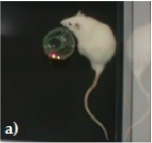
\includegraphics[width=0.17\linewidth, height=0.18\linewidth]{images/ch01/epuck/a.png} \label{figure_epuck_a}
  }
  \subfigure[接近2]{
  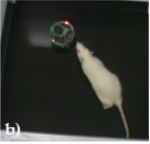
\includegraphics[width=0.17\linewidth, height=0.18\linewidth]{images/ch01/epuck/b.png} \label{figure_epuck_b}
  }
  \subfigure[嗅探]{
  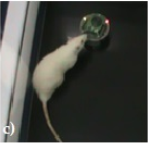
\includegraphics[width=0.17\linewidth, height=0.18\linewidth]{images/ch01/epuck/c.png} \label{figure_epuck_c}
  }
  \subfigure[跟随1]{
  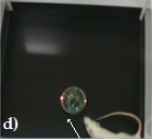
\includegraphics[width=0.17\linewidth, height=0.18\linewidth]{images/ch01/epuck/d.png} \label{figure_epuck_d}
  }
  \subfigure[跟随2]{
  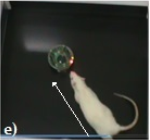
\includegraphics[width=0.17\linewidth, height=0.18\linewidth]{images/ch01/epuck/e.png} \label{figure_epuck_e}
  }\\
  \subfigure[跟随3]{
  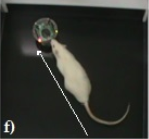
\includegraphics[width=0.17\linewidth, height=0.18\linewidth]{images/ch01/epuck/f.png} \label{figure_epuck_f}
  }
  \subfigure[攀爬]{
  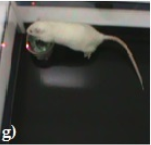
\includegraphics[width=0.17\linewidth, height=0.18\linewidth]{images/ch01/epuck/g.png} \label{figure_epuck_g}
  }
  \subfigure[梳理]{
  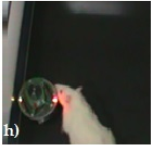
\includegraphics[width=0.17\linewidth, height=0.18\linewidth]{images/ch01/epuck/h.png} \label{figure_epuck_h}
  }
  \subfigure[自梳理]{
  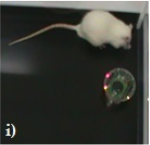
\includegraphics[width=0.17\linewidth, height=0.18\linewidth]{images/ch01/epuck/i.png} \label{figure_epuck_i}
  }
  \subfigure[躲避1]{
  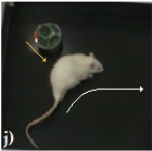
\includegraphics[width=0.17\linewidth, height=0.18\linewidth]{images/ch01/epuck/j.png} \label{figure_epuck_j}
  }\\
  \subfigure[躲避2]{
  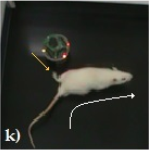
\includegraphics[width=0.17\linewidth, height=0.18\linewidth]{images/ch01/epuck/k.png} \label{figure_epuck_k}
  }
  \subfigure[探索1]{
  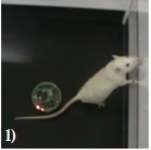
\includegraphics[width=0.17\linewidth, height=0.18\linewidth]{images/ch01/epuck/l.png} \label{figure_epuck_l}
  }
  \subfigure[探索2]{
  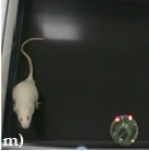
\includegraphics[width=0.17\linewidth, height=0.18\linewidth]{images/ch01/epuck/m.png} \label{figure_epuck_m}
  }
  \subfigure[不移动]{
  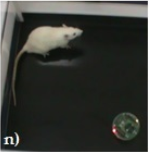
\includegraphics[width=0.17\linewidth, height=0.18\linewidth]{images/ch01/epuck/n.png} \label{figure_epuck_n}
  }
  \subfigure[镇定]{
  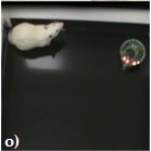
\includegraphics[width=0.17\linewidth, height=0.18\linewidth]{images/ch01/epuck/o.png} \label{figure_epuck_o}
  }
  \caption{e-puck机器人与生物鼠交互\cite{delangelortizSocialInteractionTest2016}} \label{figure_epuck}
\end{figure}

昆士兰大学的研究人员提出了一种利用轮式仿生机器鼠PiRat与生物鼠行为交互的闭环控制框架,实验中,生物鼠的运动轨迹作为PiRat控制系统的输入量,据此决定PiRat是否接近生物鼠,这一设定将生物鼠的状态作为系统输入,使得该系统具有了一定的适应性,但由于将机器鼠的动作划分为接近和远离两种模式,并未能较彻底地揭示生物鼠行为交互机理(图\ref{figure_pirat_interact})\cite{heathPiRatAutonomousFramework2018}。
\begin{figure}[htb]
  %\vspace{13pt} % 调整图片与上文的垂直距离
  \centering
  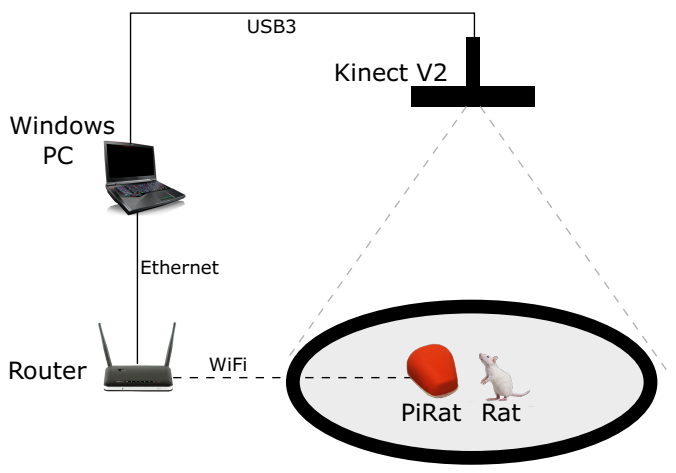
\includegraphics[width=0.5\linewidth]{images/ch01/piratintera.png}
  \caption{PiRat与生物鼠交互实验装置\cite{heathPiRatAutonomousFramework2018}}\label{figure_pirat_interact}
\end{figure}

此外还有\citeauthor{quinnWhenRatsRescue2018}研究当仿生机器鼠受困时,生物鼠是否会营救仿生机器鼠。他们利用仿生机器鼠产生“有作用”或者“无作用”的动作,并将其关入笼中,随后发现生物鼠会营救仿生机器鼠,并且倾向于营救“有作用的”仿生机器鼠(图\ref{figure_rescure})\cite{quinnWhenRatsRescue2018}。

国内对生物鼠与机器鼠的行为交互仍处于起步阶段,但利用强化学习和马尔可夫决策过程进行人机交互的训练已经得到应用。北京科技大学的\citeauthor{wangJiYuFangRenJiQiRenDeRenJiJiaoHuYuHeZuoYanJiu2015}构建了一种基于情感推理的多Agent情感决策模型,并基于情感能量理论,建立起基于HMM(Hidden Markov Model)的心境状态调节算法,该算法对于不完全和确定性知识具备较为准确的推理能力\cite{wangJiYuFangRenJiQiRenDeRenJiJiaoHuYuHeZuoYanJiu2015}。

综合以上研究,目前开展的生物鼠与仿生机器鼠行为交互实验主要聚焦于三个方面。第一,通过探究生物鼠对仿生机器鼠的反应,与对生物鼠的反应作比较,验证仿生机器鼠设计的合理性。第二,通过控制仿生机器鼠产生特定的仿鼠动作,诱使生物鼠模拟和跟随仿生机器鼠的动作,作为控制生物鼠行为的途径。第三,将仿生机器鼠的动作作为生物鼠的外部刺激,观察生物鼠对特定刺激做出的反应,研究生物鼠行为模式与外部刺激的关系。而上述三个方面均缺乏对两者长期交互的关注,使得现有研究无法适应生物鼠存在的随机性。为使机器人具备高级的社交能力,必须令其能够从所处环境中学习相关经验和知识\cite{bhaumikAIRobotics2018}。强化学习的基本思想是为代理设定学习目标,使其感知环境状态并作出决策,直到达成相应的目标\cite{ISI:000481873900002}。这一特性使得强化学习有助于解决仿生机器鼠与生物鼠交互时存在的随机性问题。